\documentclass[12pt]{article}
% REVISION NOTES %%%%%%%%%%%%%%%%%%%%%%%%%%%%%%%%%%%%%%%%%%%%
% 2008-0814 Location, Date, Time
% 2008-0814 fixed citations -- added bibliography.
%
%
\usepackage{geometry}                
\geometry{letterpaper}                   
%\geometry{landscape}                
\usepackage[parfill]{parskip}    
\usepackage{daves,fancyhdr,natbib,graphicx,dcolumn,amsmath,lastpage,url}
\usepackage{amsmath,amssymb,epstopdf,longtable}
\usepackage[final]{pdfpages}
\usepackage{paralist} 
\DeclareGraphicsRule{.tif}{png}{.png}{`convert #1 `dirname #1`/`basename #1 .tif`.png}
\pagestyle{fancy}
\lhead{CE 5333}
\lhead{CE 5366}
\rhead{SPRING 2023}
\lfoot{CE 5366 -- Cleveland}
\cfoot{Page \thepage\ of \pageref{LastPage}}
\rfoot{REVISION NO. 2}
\renewcommand\headrulewidth{0pt}
%%%%%%%%%%%%%%%%%%%%%%%%%%%%%%%%%%%%%%%%%%%%%%%%%%%%%%%
\begin{document}
\begin{center}
{\textbf{{ CE 5366-- Water Resources Management}  {Exercise Set 1}}}
\end{center}
\begingroup
\begin{tabular}{p{1in} p{5in}}
Purpose: & Uncertainty and the impact of subtle changes in consequences and costs on the decision making. Critical thinking and reading of classic documents from the literature. \\
\end{tabular}
\endgroup
%%%%%%%%%%%%%%%%%%%%%%%
\section*{\small{Exercise}}
\begin{enumerate}
\item Consider a decision (action) with the properties below \\ ~\\
\begin{tabular}{cll}
Action & Outcome & Probability \\
\hline
\hline
A & 200,000 live; 400,000 die & 100\% \\
B & 198,000 live; 402,000 die & 100\% \\
\end{tabular}\\~\\
Suppose the decision makers goal is to maximize the expected value of number of lives.
Suppose the ``cost'' to implement either action is identical.
Which action would you choose? Why?
%%%%%%%%%%%%%%%%%%%%%%%%%%%%%%
\item Consider a decision (action) with the properties below \\ ~\\
\begin{tabular}{cll}
Action & Outcome & Probability \\
\hline
\hline
A & 200,000 live; 400,000 die & 100\% \\
B & 600,000 live; 0 die & 33\% \\
~ & 0 live; 600,000 die & 66\% \\
\end{tabular}\\~\\
Suppose the decision makers goal is to maximize the expected value of number of lives.
Suppose the ``cost'' to implement either action is identical.
Which action would you choose? Why?
%%%%%%%%%%%%%%%%%%%%%%%%%%%%%%%
\item Consider a decision (action) with the properties below \\ ~\\
\begin{tabular}{cll}
Action & Outcome & Probability \\
\hline
\hline
A & 200,000 live; 400,000 die & 100\% \\
B & 600,000 live; 0 die & 33.3335\% \\
~ & 0 live; 600,000 die & 65.6665\% \\
\end{tabular}\\~\\
Suppose the decision makers goal is to maximize the expected value of number of lives.
Suppose the ``cost'' to implement either action is identical.
Which action would you choose? Why?
%%%%%%%%%%%%%%%%%%%%%%%%%%%%%%%%
\newpage
%%%%%%%%%%%%%%%%%%%%%%%%%%%%%
\item Consider a decision (action) with the properties below \\ ~\\
\begin{tabular}{cll}
Action & Outcome & Probability \\
\hline
\hline
A & 200,000 live; 400,000 die & 100\% \\
B & 198,000 live; 402,000 die & 100\% \\
\end{tabular}\\~\\
Suppose the decision makers goal is to maximize the expected value of number of lives.
Suppose the ``cost'' to implement action A has a cost, equivalent to two thousand premature deaths within one year of the action.
Which action would you choose? Why?
%%%%%%%%%%%%%%%%%%%%%%%%%%%%%%
\item Consider a decision (action) with the properties below \\ ~\\
\begin{tabular}{cll}
Action & Outcome & Probability \\
\hline
\hline
A & 200,000 live; 400,000 die & 100\% \\
B & 198,000 live; 402,000 die & 100\% \\
\end{tabular}\\~\\
Suppose the decision makers goal is to maximize the expected value of number of lives.
Suppose the ``cost'' to implement action A has a cost, equivalent to two thousand premature deaths within ten years of the action.
Which action would you choose? Why?
%%%%%%%%%%%%%%%%%%%%%%%%%%%%%%%%%
\item Did ``cost'' have an effect on \textbf{your} decision?   Did the timing of the cost of that matter?   
%\item Look up the meaning (in a battlefield medicine context) of \textbf{triage}.  Elaborate on the concept of triage as applied to the problem scenarios above.  
%\item Read ``The tragedy of the commons'' by Garrett Harding (on the class server). 
%\begin{enumerate}[a)]
%\item Write an abstract of the essay (no more than one page).
%\item Consider the National Park System.  The parks are finite, yet the number of visitors per year is generally increasing.  What system of admission would you institute for controlling access to the overcrowded parks?  Would you use a reservation system?  What basis would you use in a reservation system for selecting who is admitted?
%\item Hardin states that the morality of an act is a function of the state of the system at the time the act is performed.  List three contemporary examples of acts with little current effect such as that of plainsmen in 1800 killing a bison to eat only the tongue?
%\item The use of septic tanks for  weekend homes around Lake Tahoe was common in the 1960s.  As the shores around the lake became lined with these homes, the lake became a common sewer.  Eventually it was necessary to pass a law in California and Nevada to ban the use of septic tanks and build municipal and regional disposal systems with connecting sewer lines to each home.  Discuss the use of Lake Tahoe as a ``commons'' and suggest alternatives to a legal solution to the problem (of a common sewer).
%\end{enumerate}
\item Classify the case studies in WRSPM (pp 4-19) into dominant, secondary, and tertiary issues based on the classifications in the book:
\begin{enumerate}[a)]
\item Too much water
\item Too little water
\item Polluted water
\item Degraded ecosystem
\item Navigation
\item Erosion
\item Storage capacity loss (a.k.a ``Reservoir Issues'')
\end{enumerate}

\end{enumerate}

%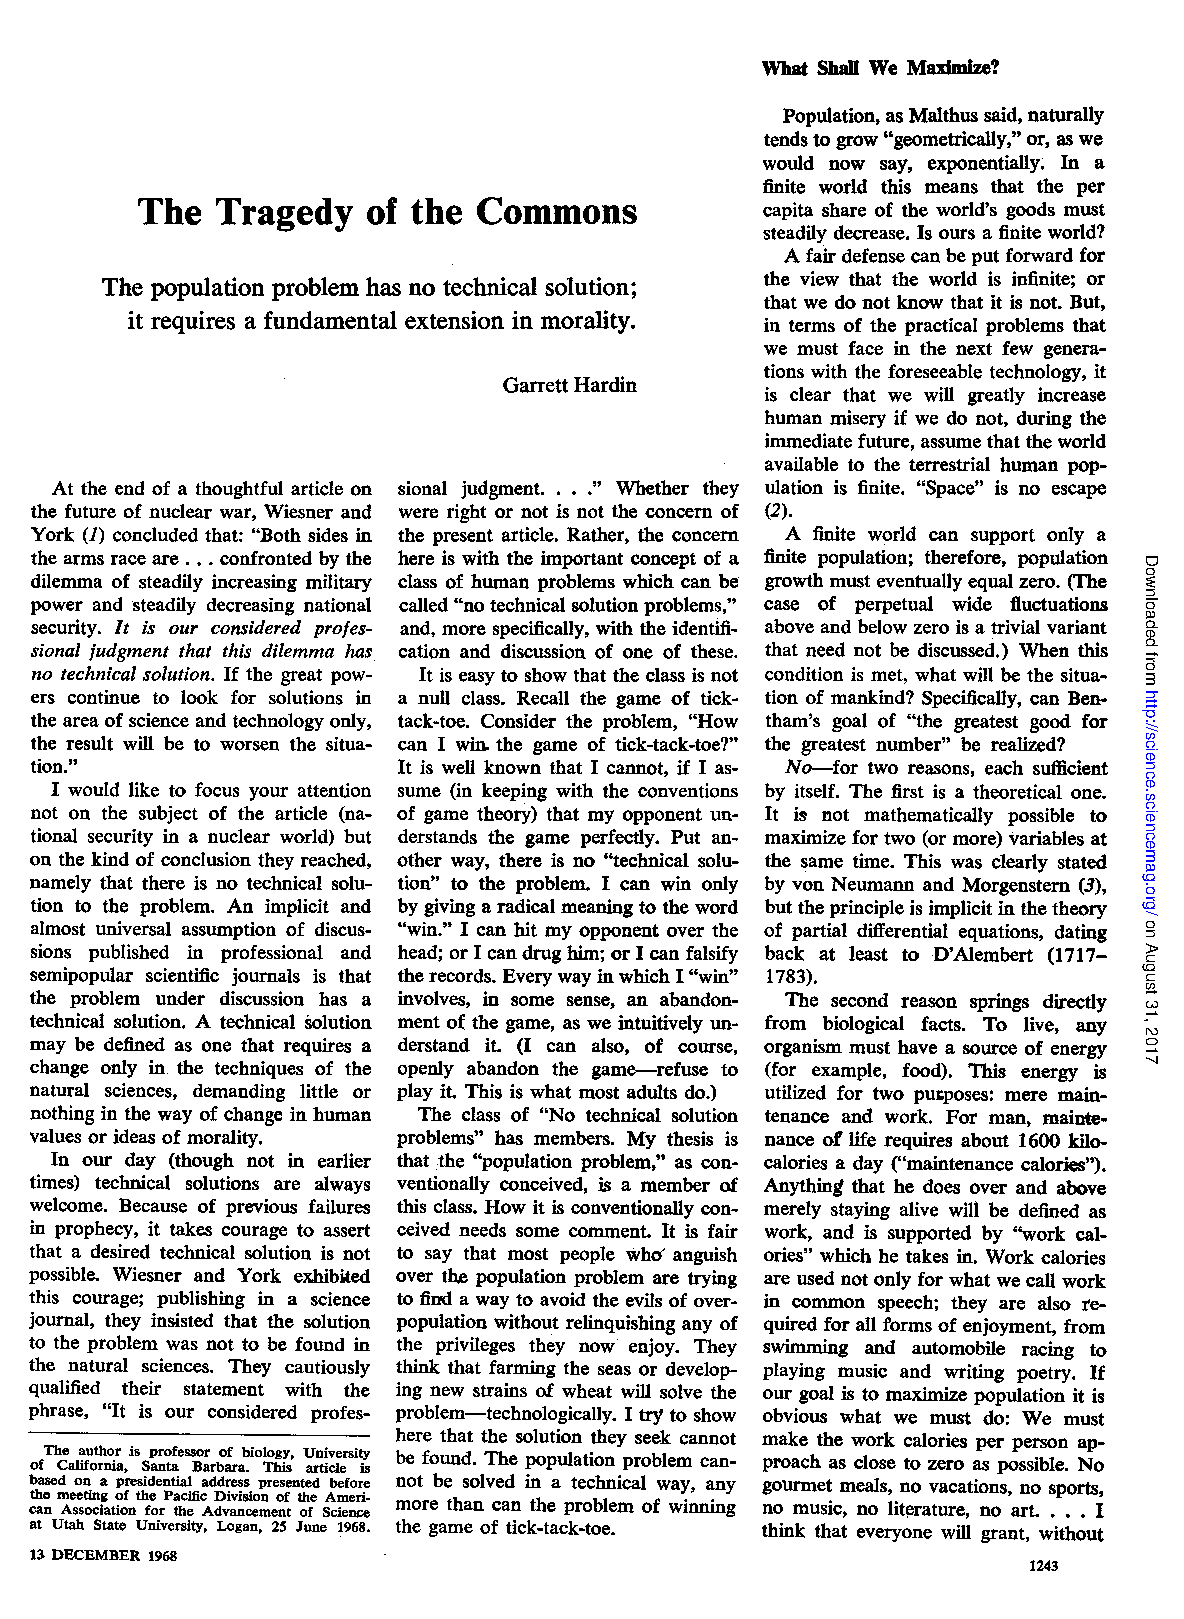
\includepdf[pages={-}]{./1243full.pdf}

\end{document}


